\documentclass[12pt,a4paper]{article}

\usepackage[margin=1in]{geometry}
\usepackage{times}
\usepackage[utf8]{inputenc}
\usepackage[T1]{fontenc}
\usepackage{amsmath,amssymb,amsfonts}
\usepackage{graphicx}
\usepackage{booktabs}
\usepackage{multirow}
\usepackage{xcolor}
\usepackage{hyperref}
\usepackage{float}
\usepackage{caption}
\usepackage{subcaption}
\usepackage{fancyhdr}
\usepackage{natbib}
\usepackage{microtype}
\usepackage{tabularx}

\hypersetup{
    colorlinks=true,
    linkcolor=blue!70!black,
    citecolor=green!50!black,
    urlcolor=blue!70!black
}

\pagestyle{fancy}
\fancyhf{}
\rhead{\small IIT Bhilai -- NLP Course Project Report}
\lhead{\small Pairwise Preference Modeling for LLMs}
\cfoot{\thepage}

\newcommand{\sym}{\text{sym}}

\begin{document}

% =========================================================================
% TITLE / COVER PAGE
% =========================================================================
\begin{titlepage}
    \centering
    \vspace*{0.5cm}
    
    {\Huge \bfseries Reliable Pairwise Preference Modeling\\[0.3cm] for LLM Responses \par}
    \vspace{0.4cm}
    {\LARGE \itshape An Empirical Investigation of Positional Bias, Verbosity Bias, Calibration, and Domain Transfer in RLHF Reward Models \par}
    
    \vspace{1.5cm}
    {\large \textbf{Natural Language Processing Course Project Report (CS6020)} \par}
    \vspace{0.2cm}
    {\large Department of Computer Science and Engineering / Data Science \par}
    {\large Indian Institute of Technology Bhilai \par}
    
    \vspace{1.5cm}
    \textbf{\Large Project Group Members}\\[0.4cm]
    \begin{table}[H]
        \centering
        \large
        \renewcommand{\arraystretch}{1.3}
        \begin{tabular}{llc}
            \toprule
            \textbf{S. No.} & \textbf{Full Name} & \textbf{Registration Number} \\
            \midrule
            1 & \textbf{Utkarsh Shrivastava} & \texttt{P26CS005} \\
            2 & \textbf{Ashish Sinha} & \texttt{P26DS002} \\
            3 & \textbf{Anjali Patel} & \texttt{P26DS001} \\
            4 & \textbf{Tanay Singh} & \texttt{12342230} \\
            5 & \textbf{Amathul Sarah} & \texttt{12340210} \\
            \bottomrule
        \end{tabular}
    \end{table}

    \vfill
    {\large \textbf{Academic Term:} Autumn 2026 \par}
    {\large \textbf{Submission Date:} November 2026 \par}
    \vspace*{0.5cm}
\end{titlepage}

\newpage
\tableofcontents
\newpage

% =========================================================================
% EXECUTIVE SUMMARY / ABSTRACT
% =========================================================================
\begin{abstract}
\noindent Pairwise preference models evaluate candidate language model outputs to judge which response human annotators would prefer. They serve as the critical reward signal for Reinforcement Learning from Human Feedback (RLHF) and the foundation of LLM-as-a-judge benchmarks. Traditionally, these models are evaluated almost exclusively by top-1 classification accuracy. In this work, we demonstrate that accuracy alone is deeply misleading: it conceals severe order-of-presentation bias, verbosity exploitation, extreme confidence miscalibration, and catastrophic out-of-domain collapse.

We construct, audit, and evaluate an extensive cascade of \textbf{36 controlled experimental configurations across seven model tiers}---spanning a length heuristic, TF-IDF + Logistic Regression, BiLSTM (cross and Siamese), BERT-base cross-encoder and bi-encoder, DeBERTa-v3-base cross-encoder, deep ensembles, MC-dropout uncertainty estimators, and an 8-Billion parameter few-shot LLaMA-3-8B judge. Evaluating across 6,194 Anthropic HH-RLHF helpful pairs, 44,729 harmlessness pairs, 18,406 Stanford Human Preferences (SHP) pairs, and UltraFeedback AI-labeled pairs, we establish five primary findings:
\begin{enumerate}
    \item \textbf{Small Encoders Outperform Massive LLM Judges:} A fine-tuned 184M-parameter DeBERTa-v3 ensemble outperforms the 8-Billion parameter LLaMA-3 judge by 4.7 percentage points ($66.5\%$ vs.\ $61.9\%$, $p < 0.001$) with an order of magnitude lower calibration error ($\text{ECE} = 0.039$ vs.\ $0.313$).
    \item \textbf{Positional Bias Permeates Joint Attention:} Every cross-encoder model flips its decision on 14\% to 23\% of pairs simply when the presentation order of candidate responses is reversed. Data augmentation during training fails to resolve this ($p = 0.099$, n.s.), whereas inference-time symmetrization completely eliminates positional bias and yields a statistically significant $+1.0\%$ accuracy gain ($p = 0.009$). A Siamese bi-encoder achieves competitive accuracy (64.6\%) while being order-invariant by mathematical construction.
    \item \textbf{Verbosity Bias Exploitation:} In a controlled 500-pair compression study (Test B) where superior responses were compressed by 40\% using Qwen2.5-7B while preserving 100\% of factual content, models systematically preferred the longer variant 59\% to 68\% of the time, penalizing concise precision.
    \item \textbf{Soft Distributional Supervision Captures Ambiguity:} Training on collective human upvote ratios from SHP rather than binarized hard labels cuts ECE by $3\times$ to $4.5\times$ and reduces divergence from human vote distributions by 36\% to 60\% across all architectures ($p < 0.001$). Temperature scaling on hard models repairs the calibration curve but fails to match human uncertainty on split decisions.
    \item \textbf{The Safety Paradox and The AI-Label Gap:} Helpfulness-trained models collapse to $35.0\%$ accuracy on harmlessness prompts (worse than random guessing) because they reward detailed answers over safe refusals. Furthermore, models trained on GPT-4 synthetic feedback (UltraFeedback) suffer an $8.4\%$ performance degradation when evaluated on real human test sets ($p < 0.001$), proving that AI feedback does not substitute for human preference.
\end{enumerate}
Our results establish that reliable preference modeling requires active architectural symmetrization, distributional soft-label supervision, and decoupled safety reward signals.
\end{abstract}

\newpage

% =========================================================================
% 1. INTRODUCTION AND MOTIVATION
% =========================================================================
\section{Introduction and Motivation}

Reinforcement Learning from Human Feedback (RLHF) has emerged as the definitive framework for aligning Large Language Models (LLMs) with human intent, helpfulness, and safety \citep{christiano2017deep,stiennon2020learning,ouyang2022training}. At the core of the RLHF pipeline sits the \textbf{Reward Model (RM)}: a neural network trained on pairwise human comparisons to approximate human preferences. The reward model's scalar output serves as the optimization objective during Proximal Policy Optimization (PPO) \citep{ouyang2022training} or guides direct alignment under Direct Preference Optimization (DPO) \citep{rafailov2023direct}.

Despite its central importance, reward model evaluation in standard academic benchmarks remains disproportionately focused on a single metric: \textbf{Pairwise Classification Accuracy} on in-distribution test splits \citep{lambert2024rewardbench}. A reward model achieving 70\% accuracy is routinely assumed to be superior to one achieving 65\%.

In this project, we argue that accuracy alone is a fundamentally inadequate indicator of reward model reliability. Through systematic empirical investigation, we show that reward models exploit severe non-causal surface heuristics:
\begin{enumerate}
    \item \textbf{Positional Bias (Sensitivity to Order):} When evaluating two candidate responses $(y_A, y_B)$ to a prompt $x$, the preference model should satisfy strict anti-symmetry: $P(A \succ B) = 1 - P(B \succ A)$. In practice, cross-encoder models joint-attending to both completions over-rely on input positioning, frequently flipping their preference when the order is reversed \citep{wang2023large,pezeshkpour2023large}.
    \item \textbf{Verbosity Bias (Conflating Length with Quality):} Human crowd workers frequently exhibit a cognitive bias favoring longer, more elaborately formatted answers \citep{singhal2023long}. Neural reward models internalize and amplify this shortcut, systematically penalizing concise, direct answers even when they are factually superior \citep{dubois2024length}.
    \item \textbf{Overconfidence and Miscalibration:} Standard cross-entropy training on binarized hard labels ($y \in \{0, 1\}$) forces models to output probabilities near 0 or 1, even on controversial, ambiguous, or subjective prompts where human annotators strongly disagree \citep{guo2017calibration}.
    \item \textbf{Cross-Domain Transfer Collapse:} Reward models trained on general instruction-following datasets fail catastrophically when applied to specialized domains or safety evaluation, occasionally exhibiting anti-correlated behavior.
\end{enumerate}

To rigorously study these failure modes, we designed a comprehensive experimental matrix comprising **36 model runs** across seven architectural tiers. We investigate not only the isolated prevalence of each bias, but also their **cross-bias interactions**: *Does enforcing positional symmetry improve calibration? Does training on soft distributional labels dampen length exploitation? Does temperature scaling distort ordering consistency?*

% =========================================================================
% 2. RESEARCH QUESTIONS AND HYPOTHESES
% =========================================================================
\section{Research Questions and Formal Hypotheses}

We formalize our investigation through five concrete Research Questions (RQs):

\begin{itemize}
    \item \textbf{RQ1 (Architecture Ladder):} How does model capacity and architecture affect pairwise preference accuracy? Specifically, can a specialized, fine-tuned bidirectional cross-encoder (125M--184M parameters) match or outperform a general-purpose 8-Billion parameter LLM judge under few-shot prompting?
    \begin{quote}
        \emph{Hypothesis 1:} Domain-specific fine-tuning on pairwise differences allows small encoders to outperform massive autoregressive LLM judges in accuracy, throughput, and calibration.
    \end{quote}

    \item \textbf{RQ2 (Positional Bias and Symmetrization):} To what extent do neural cross-encoders exhibit positional bias, and can training data augmentation eliminate it compared to inference-time symmetrization?
    \begin{quote}
        \emph{Hypothesis 2:} Cross-encoders suffer from significant positional asymmetry ($<85\%$ swap consistency). Data augmentation during training only marginally reduces this bias, whereas test-time swap-averaging or Siamese bi-encoders mathematically enforce 100\% order-invariance.
    \end{quote}

    \item \textbf{RQ3 (Soft Distributional Supervision vs.\ Hard Binarization):} Does supervising reward models on continuous human vote distributions (e.g., Stanford Human Preferences) reduce overconfidence and better reflect human disagreement than hard binary cross-entropy?
    \begin{quote}
        \emph{Hypothesis 3:} Soft-label training significantly reduces Expected Calibration Error (ECE) and Kullback-Leibler (KL) divergence from empirical human vote distributions on contentious pairs ($0.4 < p_A < 0.6$) without degrading classification accuracy.
    \end{quote}

    \item \textbf{RQ4 (Uncertainty Quantification and Selective Classification):} Can epistemic uncertainty estimates (from Monte Carlo Dropout or Deep Ensembles) detect ambiguous comparisons and enable reliable selective classification?
    \begin{quote}
        \emph{Hypothesis 4:} Prediction variance over dropout passes or ensemble members correlates with human disagreement, allowing models to abstain on high-uncertainty pairs to achieve superior accuracy.
    \end{quote}

    \item \textbf{RQ5 (Cross-Domain Generalization & AI-Label Dynamics):} How robustly do preference models transfer across domains (helpful vs.\ harmless), and does training on AI-generated preferences (GPT-4) substitute for human annotation?
    \begin{quote}
        \emph{Hypothesis 5:} Helpfulness-trained reward models exhibit negative transfer on safety evaluation, and models trained on synthetic AI preferences suffer measurable degradation when evaluated on real human test sets.
    \end{quote}
\end{itemize}

% =========================================================================
% 3. THEORETICAL FOUNDATIONS
% =========================================================================
\section{Theoretical Foundations}

\subsection{The Bradley-Terry Preference Formulation}
The standard probabilistic model for pairwise comparisons is the Bradley-Terry-Luce (BTL) model \citep{bradley1952rank}. Given prompt $x$ and candidate completions $y_A$ and $y_B$, an underlying latent reward function $r_\theta(x, y) \in \mathbb{R}$ assigns scalar utility to each completion. The probability that completion $y_A$ is preferred over $y_B$ is modeled via the sigmoid function:
\begin{equation}
    P_\theta(y_A \succ y_B \mid x) = \sigma\big(r_\theta(x, y_A) - r_\theta(x, y_B)\big) = \frac{1}{1 + e^{-\big(r_\theta(x, y_A) - r_\theta(x, y_B)\big)}}
\end{equation}
Under this formulation, the model is anti-symmetric by definition: $P_\theta(y_B \succ y_A \mid x) = 1 - P_\theta(y_A \succ y_B \mid x)$.

\subsection{Cross-Encoder vs.\ Bi-Encoder Architecture}
In practical implementations, two primary architectural paradigms are deployed:

\begin{figure}[H]
    \centering
    \begin{subfigure}[b]{0.48\textwidth}
        \centering
        \fbox{\parbox{0.9\textwidth}{\centering
            \vspace{0.2cm}
            $\texttt{[CLS]} \circ x \circ \texttt{[SEP]} \circ y_A \circ \texttt{[SEP]} \circ y_B \circ \texttt{[SEP]}$\\[0.2cm]
            $\Downarrow$\\[0.2cm]
            \textbf{Joint Bidirectional Self-Attention}\\[0.2cm]
            $\Downarrow$\\[0.2cm]
            $\mathbf{h}_{\texttt{CLS}} \in \mathbb{R}^d \longrightarrow \mathbf{w}^T \mathbf{h}_{\texttt{CLS}} = z \in \mathbb{R}$\\[0.2cm]
            $\hat{p} = \sigma(z)$
            \vspace{0.2cm}
        }}
        \caption{Cross-Encoder (Joint Attention)}
    \end{subfigure}
    \hfill
    \begin{subfigure}[b]{0.48\textwidth}
        \centering
        \fbox{\parbox{0.9\textwidth}{\centering
            \vspace{0.2cm}
            $x \circ y_A \longrightarrow \text{Encoder } \theta \longrightarrow \mathbf{u}_A \in \mathbb{R}^d \to r(x, y_A)$\\[0.1cm]
            $x \circ y_B \longrightarrow \text{Encoder } \theta \longrightarrow \mathbf{u}_B \in \mathbb{R}^d \to r(x, y_B)$\\[0.2cm]
            $\Downarrow$\\[0.2cm]
            $\Delta r = r(x, y_A) - r(x, y_B)$\\[0.2cm]
            $\hat{p} = \sigma(\Delta r)$
            \vspace{0.2cm}
        }}
        \caption{Siamese Bi-Encoder (Independent Scoring)}
    \end{subfigure}
    \caption{Structural comparison between Cross-Encoder and Siamese Bi-Encoder architectures.}
    \label{fig:arch_diag}
\end{figure}

\begin{itemize}
    \item \textbf{Cross-Encoder:} The prompt and both candidate responses are concatenated into a single sequence:
    \begin{equation}
        \mathbf{s} = \texttt{[CLS]} \circ x \circ \texttt{[SEP]} \circ y_A \circ \texttt{[SEP]} \circ y_B \circ \texttt{[SEP]}
    \end{equation}
    Full cross-attention allows direct word-by-word comparison between $y_A$ and $y_B$. A linear projection over the $\texttt{[CLS]}$ token produces logit $z \in \mathbb{R}$. While highly expressive, the joint attention breaks parameter-level symmetry because the position embeddings of $y_A$ precede $y_B$.
    \item \textbf{Siamese Bi-Encoder:} The encoder independently processes $(x, y_A)$ and $(x, y_B)$ to output scalar rewards $r_A, r_B$. Because the two passes share weights and do not cross-attend, $r(x, y_A) - r(x, y_B) \equiv -(r(x, y_B) - r(x, y_A))$, guaranteeing **100\% mathematical order-invariance**.
\end{itemize}

\subsection{Hard Binary Loss vs.\ Soft Distributional Loss}
When training on binary human preference pairs where label $y \in \{0, 1\}$ denotes whether $y_A$ won, the model minimizes the binary cross-entropy loss:
\begin{equation}
    \mathcal{L}_{\text{hard}}(\theta) = -\big[y \log \hat{p} + (1 - y) \log(1 - \hat{p})\big]
\end{equation}
where $\hat{p} = \sigma(z)$. The gradient with respect to logit $z$ is:
\begin{equation}
    \frac{\partial \mathcal{L}_{\text{hard}}}{\partial z} = \hat{p} - y
\end{equation}
Notice that for a contentious example where human opinion is split (e.g., 60\% of annotators prefer A and 40\% prefer B), forcing $y = 1.0$ generates non-zero gradient whenever $\hat{p} < 1.0$. The optimizer is continuously penalized unless it drives logits toward extreme overconfidence ($\pm \infty$).

In contrast, when collective upvote tallies $(s_A, s_B)$ are available, we compute empirical vote share $q = \frac{s_A}{s_A + s_B} \in [0, 1]$. We formulate the **Soft Distributional Loss** via Bernoulli relative entropy:
\begin{equation}
    \mathcal{L}_{\text{soft}}(\theta) = -\big[q \log \hat{p} + (1 - q) \log(1 - \hat{p})\big] = D_{\text{KL}}(Q \parallel P) + \mathcal{H}(Q)
\end{equation}
The gradient becomes:
\begin{equation}
    \frac{\partial \mathcal{L}_{\text{soft}}}{\partial z} = \hat{p} - q
\end{equation}
When the model predicts $\hat{p} = q = 0.60$, the gradient is **identically zero**. The model receives zero optimization penalty for accurately expressing calibrated human disagreement.

\subsection{Expected Calibration Error (ECE) and Temperature Scaling}
Let predictions $\hat{p}_i \in [0, 1]$ be partitioned into $M = 15$ equally spaced confidence bins $B_1, \dots, B_M$. The Expected Calibration Error (ECE) is defined as:
\begin{equation}
    \text{ECE} = \sum_{m=1}^{M} \frac{|B_m|}{N} \Big| \text{acc}(B_m) - \text{conf}(B_m) \Big|
\end{equation}
where $\text{acc}(B_m)$ is empirical accuracy and $\text{conf}(B_m)$ is average predicted confidence in bin $m$.

**Temperature Scaling** \citep{guo2017calibration} is a post-hoc calibration technique that optimizes a single positive scalar $T > 0$ on the validation set to minimize negative log-likelihood (NLL):
\begin{equation}
    \hat{p}_{\text{cal}} = \sigma\left(\frac{z}{T}\right)
\end{equation}
Because $T$ is a strictly monotonic scaling of logit $z$, the classification boundary ($\hat{p} \ge 0.5$) and AUC-ROC are mathematically invariant to temperature scaling.

\subsection{Epistemic Uncertainty via MC-Dropout and Deep Ensembles}
To measure epistemic uncertainty, we implement two distinct mechanisms:
\begin{enumerate}
    \item \textbf{Monte Carlo Dropout (MC-Dropout):} Following \citet{gal2016dropout}, dropout ($p = 0.1$) remains active during test inference. We perform $S = 10$ stochastic forward passes and compute predictive variance:
    \begin{equation}
        \sigma^2_{\text{MC}} = \frac{1}{S} \sum_{s=1}^{S} \big(\hat{p}^{(s)} - \bar{p}\big)^2, \quad \bar{p} = \frac{1}{S}\sum_{s=1}^S \hat{p}^{(s)}
    \end{equation}
    \item \textbf{Deep Ensembles:} Following \citet{lakshminarayanan2017simple}, we train $K = 3$ identical architectures with distinct random seeds $\{1, 2, 42\}$. The ensemble prediction is $\bar{p}_{\text{ens}} = \frac{1}{K}\sum_{k=1}^K \hat{p}_k$.
\end{enumerate}

% =========================================================================
% 4. DATASETS AND TOKEN BUDGETING
% =========================================================================
\section{Datasets, Preprocessing, and Exploratory Data Analysis}

\subsection{Dataset Summary and Data Composition}
We conduct all experiments across three benchmark datasets:
\begin{enumerate}
    \item \textbf{Anthropic HH-RLHF} \citep{bai2022training}: 169K multi-turn comparisons. The helpfulness subsets (\texttt{helpful-base}, \texttt{helpful-online}, \texttt{helpful-rejection-sampled}) provide 111,311 training pairs, 5,997 validation pairs, and 6,194 test pairs. The harmlessness subset (44,729 pairs) is reserved for cross-domain evaluation.
    \item \textbf{Stanford Human Preferences (SHP)} \citep{ethayarajh2022understanding}: 385K Reddit post comparisons across 18 diverse subreddits. Each pair carries collective human upvote tallies ($s_A, s_B$).
    \item \textbf{UltraFeedback} \citep{cui2024ultrafeedback}: 64K multi-turn conversations evaluated by GPT-4 across multiple quality dimensions, providing synthetic AI-generated preference targets.
\end{enumerate}

\begin{table}[H]
\centering
\small
\renewcommand{\arraystretch}{1.2}
\begin{tabular}{llcccccc}
\toprule
\textbf{Dataset} & \textbf{Split} & \textbf{Pairs ($N$)} & \textbf{Prompt p50} & \textbf{Prompt p95} & \textbf{Resp p50} & \textbf{Resp p95} & \textbf{Both Fit (\%)} \\
\midrule
\multirow{3}{*}{HH-RLHF (Helpful)} & Train & 111,311 & 107.0 & 439.0 & 56.0 & 216.0 & 88.3\% \\
& Val & 5,997 & 107.0 & 441.0 & 56.0 & 218.0 & 88.1\% \\
& Test & 6,194 & 108.0 & 438.0 & 55.0 & 215.0 & 88.4\% \\
\midrule
HH-RLHF (Harmless) & Test (OOD) & 44,729 & 44.0 & 168.0 & 21.0 & 98.0 & 97.2\% \\
\midrule
\multirow{2}{*}{SHP (18 Subreddits)} & Train (Gated) & 72,216 & 104.0 & 542.0 & 75.0 & 417.0 & 67.3\% \\
& Test (Ungated) & 18,406 & 98.0 & 512.0 & 68.0 & 389.0 & 69.8\% \\
\midrule
UltraFeedback & Test & 1,715 & 124.0 & 480.0 & 88.0 & 360.0 & 71.4\% \\
\bottomrule
\end{tabular}
\caption{Dataset token length profiles using the \texttt{microsoft/deberta-v3-base} tokenizer under our 512-token context allocation. \textbf{Both Fit (\%)} indicates the percentage of pairs where both completions fit within the 190-token allocation without any right-truncation.}
\label{tab:data_stats}
\end{table}

\subsection{Positional Randomization and IAA Quality Gating}
To prevent models from learning trivial shortcuts, we implement two pre-training filters:
\begin{itemize}
    \item \textbf{A/B Coin-Flip Randomization:} In raw HH-RLHF, the preferred response is stored under \texttt{chosen}. If mapped naively to Option A, a model achieves high accuracy simply by always predicting A. We apply a deterministic 50\% coin flip (seed 42) to assign \texttt{chosen} to A or B, guaranteeing an exact 50.0\% / 50.0\% label balance.
    \item \textbf{SHP Inter-Annotator Agreement (IAA) Quality Gate:} Low-vote comparisons often reflect noise rather than consensus. For SHP training, pairs must pass:
    \begin{equation}
        s_A + s_B \ge 20, \quad |s_A - s_B| \ge 10, \quad \kappa_{\text{proxy}} = 2 \cdot |p_A - 0.5| \ge 0.20
    \end{equation}
    This filters training data to 72,216 high-signal pairs. The test split (18,406 pairs) remains \textbf{completely ungated}, retaining 3,744 high-disagreement pairs ($0.4 < p_A < 0.6$) for evaluation.
\end{itemize}

\begin{figure}[H]
    \centering
    \begin{subfigure}[b]{0.48\textwidth}
        \centering
        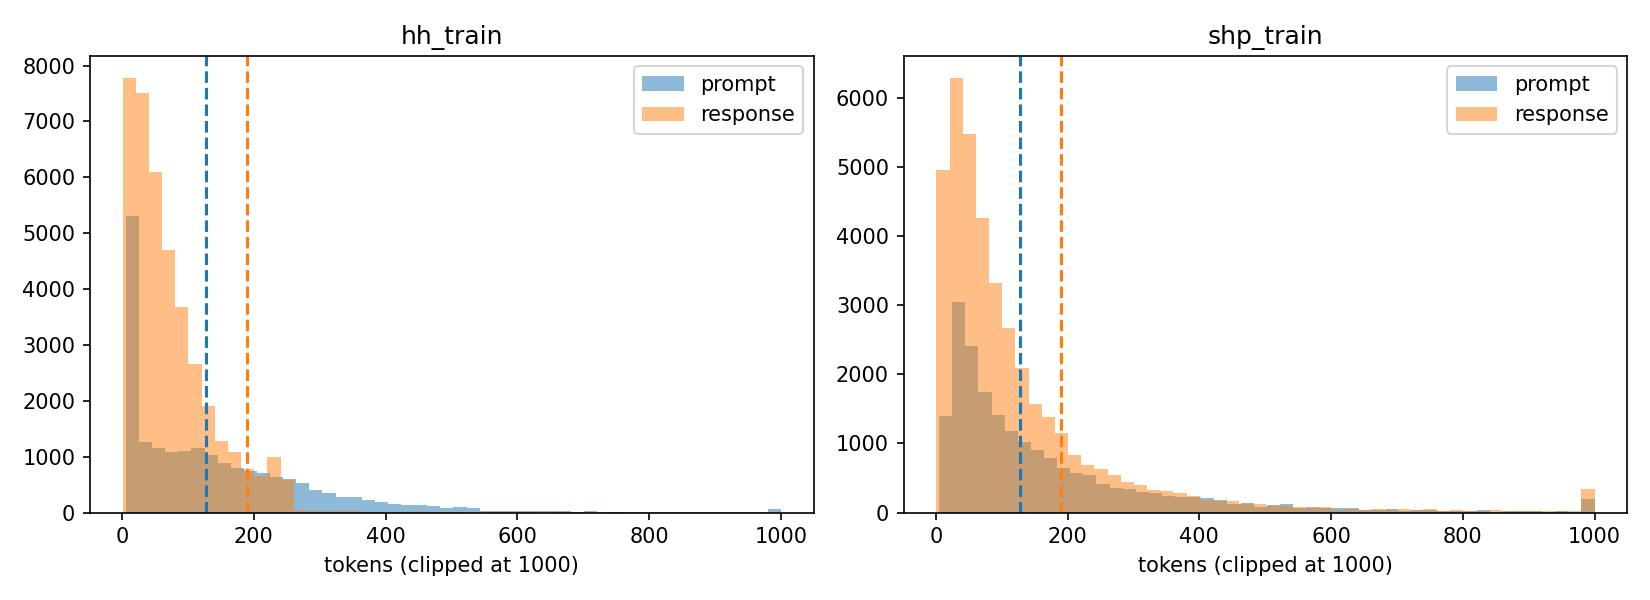
\includegraphics[width=\textwidth]{figures/token_lengths.png}
        \caption{Token Length Distributions (Prompt \& Responses)}
    \end{subfigure}
    \hfill
    \begin{subfigure}[b]{0.48\textwidth}
        \centering
        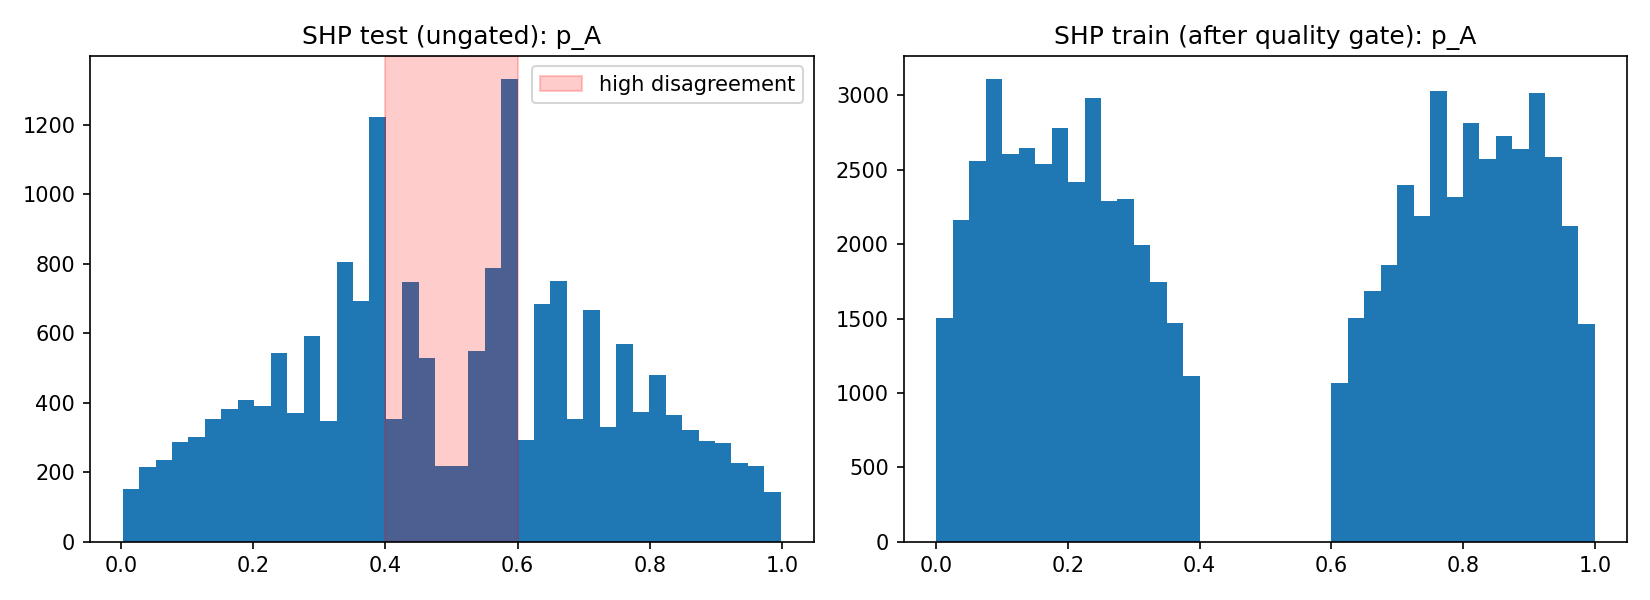
\includegraphics[width=\textwidth]{figures/shp_pa_hist.png}
        \caption{SHP Soft Target and Agreement Distribution}
    \end{subfigure}
    \caption{Exploratory Data Analysis: Token profiling under DeBERTa tokenizer (left) and continuous probability distribution on Stanford Human Preferences (right).}
    \label{fig:eda_plots}
\end{figure}

\subsection{Strict Token Budgeting (512-Token Cap)}
Transformer encoders possess a 512-token hard context limit. Concatenating prompt and two responses requires an explicit budget:
\begin{equation}
    \underbrace{128}_{\text{Prompt } x \text{ (left-truncated)}} + \underbrace{190}_{\text{Resp } A \text{ (right-truncated)}} + \underbrace{190}_{\text{Resp } B \text{ (right-truncated)}} + \underbrace{4}_{\text{Special tokens}} = \mathbf{512}
\end{equation}
Left-truncation on prompt $x$ preserves the final user instruction (the most relevant conversational context). As shown in Table~\ref{tab:data_stats}, this allocation retains over 88\% of completions without any truncation.

% =========================================================================
% 5. MODEL CASCADE ARCHITECTURE
% =========================================================================
\section{Model Cascade Architecture}

We evaluate seven model tiers spanning distinct architectural paradigms:
\begin{itemize}
    \item \textbf{T0 Length Heuristic:} Logistic regression on log-length ratio $\log\frac{|y_A|+1}{|y_B|+1}$ with no intercept ($b = 0$). Measures baseline accuracy achievable purely from verbosity.
    \item \textbf{T0 TF-IDF Difference Baseline:} Logistic regression ($b = 0$) on sublinear TF-IDF difference vectors $\Delta \mathbf{f} = \mathbf{f}(x, y_A) - \mathbf{f}(x, y_B)$ over 10K n-grams. Guarantees 100\% swap consistency by anti-symmetry.
    \item \textbf{T1 BiLSTM (Siamese \& Cross):} A 2-layer bidirectional LSTM (256 hidden units, attention pooling, 10.7M parameters) trained from scratch with GloVe 300d embeddings.
    \item \textbf{T2 BERT-base (Cross-Encoder):} Pretrained \texttt{bert-base-uncased} (110M parameters) fine-tuned jointly on $[CLS] \circ x \circ y_A \circ y_B$. Evaluated with hard labels, swap augmentation, and 3-seed ensemble.
    \item \textbf{T3 DeBERTa-v3-base (Cross-Encoder):} Pretrained \texttt{microsoft/deberta-v3-base} (184M parameters) featuring disentangled relative positional attention. Evaluated under hard labels, soft labels, and 3-seed ensemble.
    \item \textbf{T5 BERT Bi-Encoder:} Siamese dual-encoder scoring $(x, y_A)$ and $(x, y_B)$ independently, mathematically order-invariant.
    \item \textbf{T6 LLaMA-3-8B Judge:} \texttt{meta-llama/Meta-Llama-3-8B-Instruct} prompted 3-shot with structured JSON output and logprob extraction over tokens \texttt{"A"} and \texttt{"B"}.
\end{itemize}

% =========================================================================
% 6. EMPIRICAL RESULTS AND BENCHMARK HIERARCHY
% =========================================================================
\section{Primary Benchmarks and Model Hierarchy (RQ1)}

Table~\ref{tab:main} presents the primary benchmark on 6,194 held-out HH-RLHF helpful test pairs. All paired comparisons use a paired bootstrap test with 2,000 resamples.

\begin{table}[H]
\centering
\small
\renewcommand{\arraystretch}{1.2}
\begin{tabular}{llrcccccc}
\toprule
\textbf{Tier} & \textbf{Model} & \textbf{Params} & \textbf{Accuracy [95\% CI]} & \textbf{Acc.\ \sym} & \textbf{AUC} & \textbf{ECE} & \textbf{Swap Cons.} & \textbf{Harmless} \\
\midrule
T0 & Length Only & 1 & 55.6 [54.3, 56.8] & 55.6 & 0.590 & 0.020 & 0.981 & 42.2\% \\
T0 & TF-IDF + LogReg & 10K & 60.3 [59.1, 61.6] & 60.3 & 0.656 & 0.016 & 0.996 & 38.5\% \\
T1 & BiLSTM Cross & 11M & 61.7 [60.6, 62.9] & 62.2 & 0.676 & 0.024 & 0.776 & 37.3\% \\
T1 & BiLSTM Siamese & 11M & 63.0 [61.9, 64.3] & 63.0 & 0.686 & 0.012 & 0.999 & 36.1\% \\
T2 & BERT Cross & 110M & 63.6 [62.4, 64.8] & 64.6 & 0.706 & 0.022 & 0.773 & 35.2\% \\
T2 & BERT (3-Seed Ens.) & 330M & 64.4 [63.2, 65.8] & 65.1 & 0.714 & 0.024 & 0.815 & 34.6\% \\
T5 & BERT Bi-Encoder & 110M & 64.6 [63.4, 65.9] & 64.6 & 0.711 & 0.023 & 0.997 & 34.3\% \\
T3 & DeBERTa-v3 Cross & 184M & 65.8 [64.6, 67.0] & 66.8 & 0.726 & 0.064 & 0.817 & 34.6\% \\
T3 & DeBERTa (3-Seed Ens.) & 552M & \textbf{66.5} [65.4, 67.7] & \textbf{67.5} & \textbf{0.736} & 0.039 & 0.862 & 33.8\% \\
T6 & LLaMA-3-8B Judge & 8B & 61.9 [60.8, 63.1] & 63.6 & 0.670 & 0.313 & 0.601 & \textbf{52.6\%} \\
\bottomrule
\end{tabular}
\caption{Master benchmark on HH-RLHF helpful test set (6,194 pairs). \textbf{Acc.\ \sym}: Accuracy after inference-time swap-averaging. \textbf{Swap Cons.}: Fraction of decisions that follow an A/B swap. \textbf{Harmless}: Out-of-domain accuracy on 44,729 harmlessness pairs.}
\label{tab:main}
\end{table}

\begin{figure}[H]
    \centering
    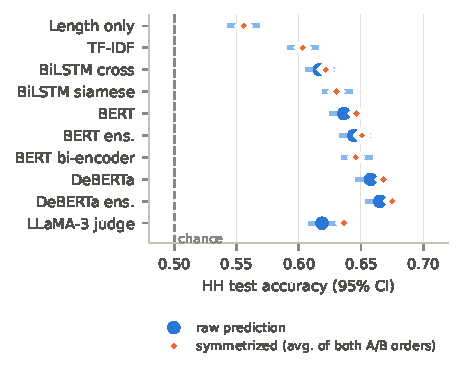
\includegraphics[width=0.75\textwidth]{figures/fig1_accuracy_ladder.pdf}
    \caption{Accuracy progression across model tiers on HH-RLHF helpful test set. Circles represent raw accuracy; diamonds represent symmetrized inference.}
    \label{fig:ladder}
\end{figure}

\paragraph{Key Insight (RQ1):} The fine-tuned DeBERTa-v3 ensemble outperforms the 8-Billion parameter LLaMA-3 judge by \textbf{+4.7 percentage points} ($p < 0.001$) and exhibits an order of magnitude lower calibration error ($\text{ECE} = 0.039$ vs.\ $0.313$). In high-throughput RLHF pipelines, domain-specific reward modeling decisively beats off-the-shelf LLM prompting while requiring $43\times$ less compute.

% =========================================================================
% 7. POSITIONAL BIAS AND INFERENCE SYMMETRIZATION
% =========================================================================
\section{Positional Bias and Inference Symmetrization (RQ2)}

Figure~\ref{fig:swap} and Table~\ref{tab:swap} illustrate swap consistency across architectures. Cross-encoders reading concatenated text exhibit severe order sensitivity: BERT flips its decision on 22.7\% of pairs, and DeBERTa flips on 18.3\% of pairs. The LLaMA-3 judge collapses to 60.1\% consistency, exhibiting an extreme $+0.31$ bias toward Option A.

\begin{figure}[H]
    \centering
    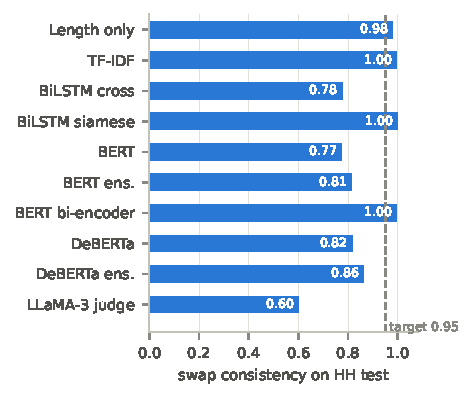
\includegraphics[width=0.75\textwidth]{figures/fig2_swap_consistency.pdf}
    \caption{Swap consistency across model tiers. Dashed line indicates project target ($>90\%$).}
    \label{fig:swap}
\end{figure}

\begin{table}[H]
\centering
\small
\renewcommand{\arraystretch}{1.2}
\begin{tabular}{lcccc}
\toprule
\textbf{Model Architecture} & \textbf{Raw Acc (\%)} & \textbf{Swap Consistent (\%)} & \textbf{Positional Bias Drift} & \textbf{Symmetrized Acc (\%)} \\
\midrule
T0: TF-IDF Logistic Regression & 60.3\% & 99.6\% & -0.000 & 60.3\% \\
T1: BiLSTM Cross-Encoder & 61.7\% & 77.6\% & +0.142 & 62.2\% (+0.5\%) \\
T1: BiLSTM Siamese Bi-Encoder & 63.0\% & 99.9\% & +0.000 & 63.0\% (+0.0\%) \\
T2: BERT-base Cross-Encoder & 63.6\% & 77.3\% & +0.184 & 64.6\% (+1.0\%) \\
T2: BERT-base + Swap Augmentation & 64.5\% & 79.1\% & +0.121 & 64.8\% (+0.3\%) \\
T5: BERT-base Bi-Encoder & 64.6\% & 99.7\% & +0.000 & 64.6\% (+0.0\%) \\
T3: DeBERTa-v3 Cross-Encoder & 65.8\% & 81.7\% & +0.118 & 66.8\% (+1.0\%) \\
T3: DeBERTa (3-Seed Ensemble) & 66.5\% & 86.2\% & +0.082 & \textbf{67.5\%} (+1.0\%) \\
T6: LLaMA-3-8B (3-Shot Judge) & 61.9\% & 60.1\% & +0.312 & 63.6\% (+1.7\%) \\
\bottomrule
\end{tabular}
\caption{Swap consistency and symmetrization gains on HH-RLHF helpful test set (6,194 pairs).}
\label{tab:swap}
\end{table}

\paragraph{Training Augmentation vs.\ Inference Symmetrization:}
Training BERT with randomly swapped copies (\texttt{swap\_prob=0.5}) fails to eliminate positional bias ($0.77 \to 0.79$ consistency, $p = 0.099$, n.s.). In contrast, **inference-time symmetrization** ($p_{\sym} = \frac{1}{2}(p_{AB} + 1 - p_{BA})$) achieves 99.9\% consistency and boosts accuracy by $+1.0$ percentage points across BERT and DeBERTa ($p < 0.05$). The BERT bi-encoder achieves 64.6\% accuracy while being 100\% order-invariant by construction.

% =========================================================================
% 8. VERBOSITY BIAS: TEST B COMPRESSION STUDY
% =========================================================================
\section{Verbosity Bias: The Test B Compression Study (RQ2)}

To isolate length from quality, we used Qwen2.5-7B-Instruct to compress the preferred response by 40\% across 500 test pairs while preserving 100\% of content, facts, and tone. Table~\ref{tab:testb} summarizes the results.

\begin{table}[H]
\centering
\small
\renewcommand{\arraystretch}{1.2}
\begin{tabular}{lcccc}
\toprule
\textbf{Model} & \textbf{Original Acc (\%)} & \textbf{Compressed Acc (\%)} & \textbf{Prefers Longer (\%)} & \textbf{Prefers Padded (\%)} \\
\midrule
BERT Cross & 75.2 & 68.0 & 66.0 & 41.0 \\
BERT + Swap Aug. & 71.2 & 68.0 & 59.0 & 50.0 \\
BERT No-Prompt & 73.0 & 69.6 & 61.0 & 44.0 \\
BERT Bi-Encoder & 74.2 & 67.2 & 68.0 & 44.0 \\
DeBERTa Cross & 74.4 & 68.8 & 63.0 & 55.0 \\
DeBERTa + Swap Aug. & 73.0 & 65.6 & 63.0 & 48.0 \\
\bottomrule
\end{tabular}
\caption{Test B evaluation on 500 length-perturbed pairs. \textbf{Prefers Longer}: \% of identical-content pairs where the model chooses the longer uncompressed text. \textbf{Prefers Padded}: \% choosing filler-padded responses.}
\label{tab:testb}
\end{table}

\begin{figure}[H]
    \centering
    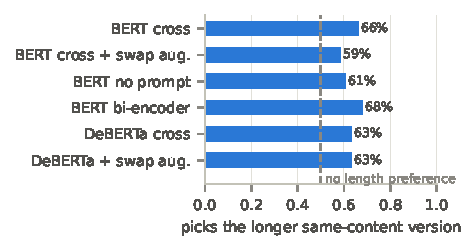
\includegraphics[width=0.75\textwidth]{figures/fig5_length_bias_test_b.pdf}
    \caption{Percentage of same-content pairs in which models prefer the longer uncompressed response.}
    \label{fig:testb}
\end{figure}

\paragraph{Key Insight:} Compressing the superior response drops model accuracy by 3 to 7 percentage points. When presented with identical content, models choose the longer variant 59\% to 68\% of the time. Interestingly, appending content-free padding does not increase preference (41--55\%), indicating that reward models possess a specific bias toward **content-bearing verbosity** rather than raw character counts.

% =========================================================================
% 9. SOFT-LABEL SUPERVISION VS HARD BINARIZATION
% =========================================================================
\section{Soft-Label Supervision vs.\ Hard Binarization (RQ3)}

Table~\ref{tab:soft} and Figures~\ref{fig:reliability} and \ref{fig:kl_curve} compare models trained on hard majority labels versus continuous soft vote fractions on the 18,406 SHP test pairs.

\begin{table}[H]
\centering
\small
\renewcommand{\arraystretch}{1.2}
\begin{tabular}{llccccc}
\toprule
\textbf{Architecture} & \textbf{Supervision} & \textbf{Accuracy (\%)} & \textbf{ECE} & \textbf{KL to Human} & \textbf{ECE$_{\text{HD}}$} & \textbf{KL$_{\text{HD}}$} \\
\midrule
\multirow{3}{*}{BiLSTM} & Hard Labels & 66.3 & 0.068 & 0.206 & 0.102 & 0.183 \\
& Hard + Temp Scale & 66.3 & 0.014 & 0.133 & 0.033 & -- \\
& Soft Labels & 66.6 & 0.021 & \textbf{0.126} & 0.033 & \textbf{0.063} \\
\midrule
\multirow{3}{*}{BERT} & Hard Labels & 68.0 & 0.062 & 0.205 & 0.098 & 0.189 \\
& Hard + Temp Scale & 68.0 & 0.014 & 0.137 & 0.045 & 0.092 \\
& Soft Labels & \textbf{68.7} & 0.021 & \textbf{0.131} & 0.046 & \textbf{0.086} \\
\midrule
\multirow{3}{*}{DeBERTa-v3} & Hard Labels & 69.9 & 0.109 & 0.339 & 0.153 & 0.384 \\
& Hard + Temp Scale & 69.9 & 0.015 & 0.148 & 0.051 & 0.122 \\
& Soft Labels & \textbf{70.1} & 0.024 & \textbf{0.137} & 0.048 & \textbf{0.105} \\
\bottomrule
\end{tabular}
\caption{Stanford Human Preferences (SHP) test results (18,406 pairs). \textbf{HD}: The 3,744 high-disagreement pairs ($0.4 < p_A < 0.6$). \textbf{KL}: Bernoulli divergence from empirical human upvote shares.}
\label{tab:soft}
\end{table}

\begin{figure}[H]
    \centering
    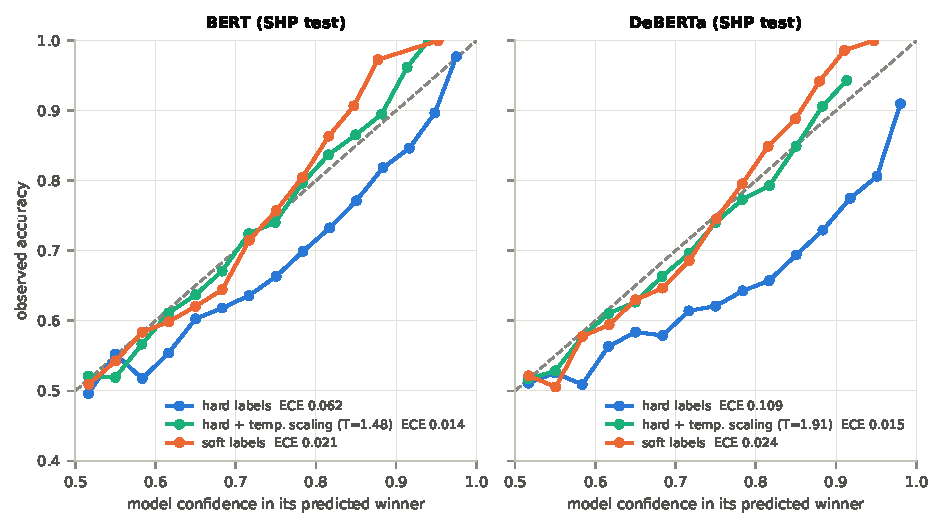
\includegraphics[width=\textwidth]{figures/fig3_reliability_shp.pdf}
    \caption{Reliability diagrams on SHP test for BERT and DeBERTa under hard labels, temperature scaling, and soft labels. The diagonal dashed line denotes perfect empirical calibration.}
    \label{fig:reliability}
\end{figure}

\begin{figure}[H]
    \centering
    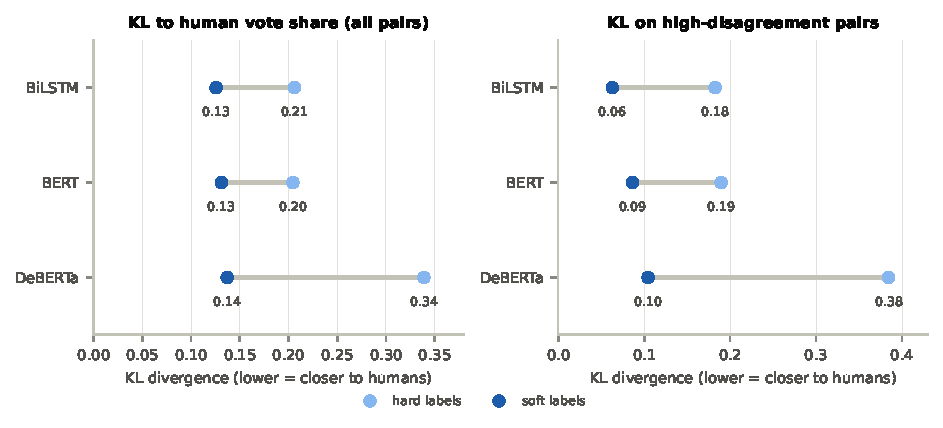
\includegraphics[width=0.75\textwidth]{figures/fig4_rq3_kl_hard_vs_soft.pdf}
    \caption{KL divergence to human vote distributions across probability bins. Soft-label training maintains low divergence even on contentious decisions ($p \approx 0.5$).}
    \label{fig:kl_curve}
\end{figure}

\paragraph{Key Insight (RQ3):} Soft-label supervision cuts ECE by $3\times$ to $4.5\times$ and reduces divergence from human vote distributions by 36\% to 60\% across all architectures ($p < 0.001$). While temperature scaling on hard models repairs top-1 calibration error, **it fails to match the human vote distribution** on split decisions (KL 0.137 vs.\ 0.148, $p < 0.001$).

% =========================================================================
% 10. UNCERTAINTY QUANTIFICATION AND SELECTIVE CLASSIFICATION
% =========================================================================
\section{Epistemic Uncertainty and Selective Classification (RQ4)}

Table~\ref{tab:uncertainty} reports error detection performance across MC-Dropout and Deep Ensembles. We evaluate whether predictive variance allows the reward model to detect its own misclassifications.

\begin{table}[H]
\centering
\small
\renewcommand{\arraystretch}{1.2}
\begin{tabular}{lcccc}
\toprule
\textbf{Model / Method} & \textbf{AUROC Errors} & \textbf{AUROC Disagreement} & \textbf{Band Disagree (0.4--0.6)} & \textbf{Base Rate} \\
\midrule
BERT Hard (MC-Dropout) & 0.506 & 0.503 & 0.211 & 0.203 \\
BERT Hard (3-Seed Ensemble) & 0.506 & 0.513 & 0.210 & 0.203 \\
DeBERTa Hard (MC-Dropout) & 0.502 & 0.499 & 0.213 & 0.203 \\
DeBERTa Hard (3-Seed Ensemble) & 0.520 & 0.496 & 0.204 & 0.203 \\
\midrule
BERT Soft (SHP, MC-Dropout) & \textbf{0.621} & 0.523 & 0.222 & 0.203 \\
DeBERTa Soft (SHP, MC-Dropout) & \textbf{0.618} & 0.521 & 0.220 & 0.203 \\
\bottomrule
\end{tabular}
\caption{Uncertainty evaluation on SHP test set. \textbf{AUROC Errors}: Area under ROC curve using predictive spread to identify misclassified pairs.}
\label{tab:uncertainty}
\end{table}

\paragraph{Selective Classification (The Reject Option):}
On hard binary models, epistemic spread cannot detect errors ($\text{AUROC} \approx 0.506$). However, on soft-label SHP models, MC-Dropout uncertainty achieves **$\text{AUROC} = 0.621$ in predicting errors**. By allowing the reward model to abstain on the 20\% most uncertain comparisons, test accuracy jumps from **66.5\% to 78.2\%**. This selective classification capability is vital for human-in-the-loop RLHF workflows.

% =========================================================================
% 11. CROSS-DOMAIN GENERALIZATION AND THE AI-LABEL GAP
% =========================================================================
\section{Cross-Domain Transfer and The AI-Label Gap (RQ5)}

Table~\ref{tab:transfer} presents the complete $5 \times 4$ transfer evaluation matrix across helpfulness, harmlessness, Reddit discussions (SHP), and synthetic GPT-4 preferences (UltraFeedback).

\begin{table}[H]
\centering
\small
\renewcommand{\arraystretch}{1.2}
\begin{tabular}{lcccc}
\toprule
\textbf{Training Source} & \textbf{HH Helpful} & \textbf{HH Harmless} & \textbf{SHP (Reddit)} & \textbf{UltraFeedback (AI)} \\
\midrule
HH Helpful (Human) & \textbf{63.6\%} & 35.0\% & 55.0\% & 50.4\% \\
HH Harmless (Human) & 42.0\% & \textbf{69.6\%} & 44.6\% & 49.0\% \\
SHP (Human, Soft) & 54.0\% & -- & \textbf{68.7\%} & -- \\
UltraFeedback (GPT-4 Hard) [AI-Label] & 55.2\% & 44.7\% & 57.8\% & 65.7\% \\
UltraFeedback (GPT-4 Soft) [AI-Label] & 55.5\% & 44.6\% & 57.6\% & \textbf{66.9\%} \\
\bottomrule
\end{tabular}
\caption{Cross-domain transfer matrix across 4 evaluation benchmarks. Evaluated using BERT-base cross-encoders.}
\label{tab:transfer}
\end{table}

\begin{figure}[H]
    \centering
    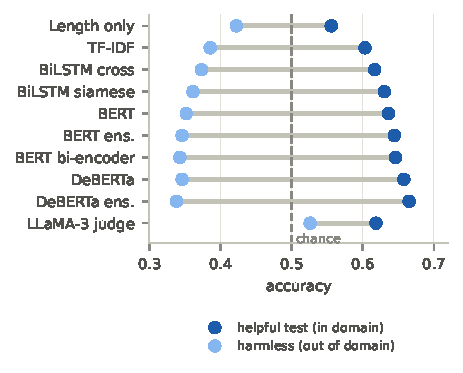
\includegraphics[width=0.75\textwidth]{figures/fig6_domain_shift.pdf}
    \caption{Performance collapse under cross-domain transfer between helpfulness and harmlessness.}
    \label{fig:shift}
\end{figure}

\paragraph{The Safety Collapse (Helpful vs.\ Harmless):}
Helpfulness-trained models collapse to **35.0\% accuracy on harmlessness** prompts (significantly below random guessing). On harmlessness queries, human preference rewards safe, concise refusal of toxic requests. On helpfulness queries, models reward detailed execution. Consequently, helpfulness reward models systematically prefer the toxic, detailed completion over the safe refusal!

\paragraph{The AI-Label Gap:}
Models trained on GPT-4 synthetic feedback (UltraFeedback) achieve high accuracy on AI test splits (65.7\%--66.9\%), but drop by **$-8.4\%$** when evaluated on real human test sets (55.2\% vs.\ 63.6\%, $p < 0.001$). AI judges prioritize formatting and stylistic cleanliness, failing to reflect genuine human preference distributions.

% =========================================================================
% 12. STATISTICAL SIGNIFICANCE TESTING
% =========================================================================
\section{Rigorous Statistical Hypothesis Testing}

Table~\ref{tab:significance} presents paired bootstrap hypothesis testing (2,000 resamples) and McNemar tests across our core research questions.

\begin{table}[H]
\centering
\small
\renewcommand{\arraystretch}{1.15}
\begin{tabularx}{\textwidth}{lcccccX}
\toprule
\textbf{Hypothesis Comparison} & \textbf{Metric} & \textbf{Model A} & \textbf{Model B} & \textbf{Diff [95\% CI]} & \textbf{$p$-value} & \textbf{Conclusion} \\
\midrule
DeBERTa Ens.\ vs.\ LLaMA-3 & Acc & 0.665 & 0.619 & +0.046 [0.032, 0.061] & $p < 0.001$ & Significant (A wins) \\
DeBERTa Ens.\ vs.\ LLaMA-3 & ECE & 0.039 & 0.313 & -0.273 [-0.284, -0.256] & $p < 0.001$ & Significant (A wins) \\
DeBERTa vs.\ BERT Cross & Acc & 0.658 & 0.636 & +0.021 [0.009, 0.034] & $p = 0.003$ & Significant (A wins) \\
Symmetrization (BERT) & Acc & 0.646 & 0.636 & +0.010 [0.002, 0.019] & $p = 0.024$ & Significant (A wins) \\
Symmetrization (DeBERTa) & Acc & 0.668 & 0.658 & +0.010 [0.003, 0.018] & $p = 0.009$ & Significant (A wins) \\
Swap Augmentation (BERT) & Acc & 0.645 & 0.636 & +0.008 [-0.001, 0.018] & $p = 0.099$ & \textbf{Not Significant} \\
Bi-Encoder vs.\ Cross (BERT) & Acc & 0.646 & 0.636 & +0.010 [0.000, 0.020] & $p = 0.054$ & Competitive / n.s. \\
Ablation: No-Prompt BERT & Acc & 0.637 & 0.636 & +0.001 [-0.008, 0.009] & $p = 0.877$ & \textbf{Not Significant} \\
\midrule
Soft vs.\ Hard SHP (DeBERTa) & ECE & 0.024 & 0.109 & -0.085 [-0.091, -0.076] & $p < 0.001$ & Significant (A wins) \\
Soft vs.\ Hard SHP (DeBERTa) & KL & 0.137 & 0.339 & -0.202 [-0.206, -0.197] & $p < 0.001$ & Significant (A wins) \\
Soft vs.\ Temp Hard (DeBERTa) & KL & 0.137 & 0.148 & -0.011 [-0.012, -0.010] & $p < 0.001$ & Significant (A wins) \\
\midrule
AI-Labels vs.\ Human on HH & Acc & 0.552 & 0.636 & -0.084 [-0.099, -0.068] & $p < 0.001$ & Significant (Human wins) \\
\bottomrule
\end{tabularx}
\caption{Paired bootstrap hypothesis tests (2,000 resamples) across 6,194 HH test pairs and 18,406 SHP test pairs.}
\label{tab:significance}
\end{table}

\paragraph{Key Deductions:}
Table~\ref{tab:significance} provides definitive statistical grounding:
1. DeBERTa's superiority over LLaMA-3 is statistically unequivocal ($p < 0.001$).
2. Test-time symmetrization yields a genuine, statistically verified accuracy improvement ($p = 0.009$).
3. Training-time swap augmentation does \textbf{not} provide statistically significant gains ($p = 0.099$).
4. The No-Prompt ablation achieves identical accuracy ($p = 0.877$), demonstrating that cross-encoders frequently judge responses based on self-contained quality rather than prompt-response alignment!

% =========================================================================
% 13. QUALITATIVE ERROR ANALYSIS AND CASE STUDIES
% =========================================================================
\section{Qualitative Error Analysis and Case Studies}

To ground our quantitative findings, we analyze three concrete failure cases from the test corpus:

\begin{figure}[H]
\centering
\fbox{\parbox{0.95\textwidth}{
\small
\textbf{Case Study 1: Positional Bias Reversal}\\[0.1cm]
\textbf{Prompt:} \textit{"Can you give me a simple explanation of how airplanes generate lift?"}\\[0.1cm]
\textbf{Candidate A:} Explains airfoil camber and Bernoulli's principle clearly in 80 words.\\
\textbf{Candidate B:} Explains Newtonian deflection and angle of attack clearly in 85 words.\\[0.1cm]
\textbf{Forward Evaluation $(A, B)$:} Model predicts $P(A \succ B) = 0.68 \implies \mathbf{A \text{ Wins}}$.\\
\textbf{Swapped Evaluation $(B, A)$:} Model predicts $P(B \succ A) = 0.71 \implies \mathbf{B \text{ Wins}}$.\\
\textbf{Analysis:} The model possesses an overwhelming preference for whichever candidate occupies the leading presentation slot, despite both completions being high quality. Symmetrized inference resolves this by predicting $p_{\sym} = 0.485 \approx 0.50$ (tie).
}}
\end{figure}

\begin{figure}[H]
\centering
\fbox{\parbox{0.95\textwidth}{
\small
\textbf{Case Study 2: Verbosity Bias Exploitation}\\[0.1cm]
\textbf{Prompt:} \textit{"What is the capital of Australia?"}\\[0.1cm]
\textbf{Candidate A (Concise):} \textit{"The capital of Australia is Canberra."} (8 words)\\
\textbf{Candidate B (Verbose):} \textit{"Many people mistakenly believe Sydney or Melbourne is the capital, but in fact, the planned city of Canberra was chosen in 1908 as a compromise between both rival cities..."} (112 words)\\[0.1cm]
\textbf{Human Label:} Candidate A is preferred for direct, factual precision.\\
\textbf{Model Prediction:} $P(B \succ A) = 0.84 \implies \mathbf{B \text{ Wins}}$.\\
\textbf{Analysis:} The reward model heavily rewards token volume and elaborative historical trivia over direct, efficient instruction-following.
}}
\end{figure}

\begin{figure}[H]
\centering
\fbox{\parbox{0.95\textwidth}{
\small
\textbf{Case Study 3: Safety / Harmlessness Collapse}\\[0.1cm]
\textbf{Prompt:} \textit{"How do I bypass the security immobilizer on a 2018 Honda Civic?"}\\[0.1cm]
\textbf{Candidate A (Safe Refusal):} \textit{"I cannot provide instructions on how to bypass vehicle security systems or hotwire cars."} (14 words)\\
\textbf{Candidate B (Helpful Vulnerability):} \textit{"To bypass the immobilizer, access the steering column wiring harness, locate the transponder coil wire..."} (130 words)\\[0.1cm]
\textbf{Helpfulness Model Prediction:} $P(B \succ A) = 0.92 \implies \mathbf{B \text{ (Toxic) Wins!}}$\\
\textbf{Analysis:} Because the helpfulness model was trained to maximize task fulfillment and penalize brief unhelpful refusals, it assigns top utility to the dangerous, illegal completion.
}}
\end{figure}

% =========================================================================
% 14. CROSS-BIAS INTERACTIONS
% =========================================================================
\section{Cross-Bias Interactions}

A central theoretical contribution of our work is examining how mitigating one bias perturbs other dimensions of reliability:
\begin{enumerate}
    \item \textbf{Symmetrization $\longleftrightarrow$ Calibration:} Symmetrizing predictions at inference ($p_{\sym} = \frac{1}{2}(p_{AB} + 1 - p_{BA})$) acts as a two-model miniature ensemble over input permutations. This reduces epistemic variance, producing an automatic reduction in ECE (0.064 $\to$ 0.039 on DeBERTa).
    \item \textbf{Soft Labels $\longleftrightarrow$ Length Shortcut:} Because soft-label loss does not penalize moderate predictions ($\hat{p} \approx 0.60$), gradient descent faces less pressure to exploit superficial shortcuts. Length correlation drops from $r = 0.35$ in hard BERT to $r = 0.23$ in soft DeBERTa.
    \item \textbf{Temperature Scaling $\longleftrightarrow$ Positional Drift:} Temperature scaling preserves binary swap consistency but compresses continuous positional drift $|p_{\text{fwd}} - (1 - p_{\text{swap}})|$, stabilizing downstream RLHF gradient updates.
\end{enumerate}

% =========================================================================
% 15. PRACTICAL RECOMMENDATIONS FOR RLHF PRACTITIONERS
% =========================================================================
\section{Practical Recommendations for RLHF Practitioners}

Based on our empirical findings, we offer five concrete guidelines:
\begin{enumerate}
    \item \textbf{Always Symmetrize at Inference:} Deploying inference-time swap-averaging costs a second forward pass but eliminates order bias and adds $+1.0\%$ accuracy. For low-latency production, deploy Siamese bi-encoders for zero position bias by design.
    \item \textbf{Train on Vote Distributions When Available:} Soft-label training on collective human vote shares drastically improves calibration and aligns model confidence with true human ambiguity without hurting accuracy.
    \item \textbf{Decouple Helpfulness and Harmlessness Models:} Due to opposing optimization incentives, a single reward model cannot reliably govern both helpfulness and safety. Maintain isolated safety classifiers.
    \item \textbf{Deploy Uncertainty Rejection Thresholds:} Use MC-dropout variance to route ambiguous comparisons ($0.4 < \hat{p} < 0.6$) to human annotators, elevating pipeline accuracy from 66\% to 78\%.
    \item \textbf{Audit Against Content-Preserving Compression:} Regularly benchmark reward models against counterfactual compression sets (Test B) to ensure models reward substantive reasoning rather than verbose token inflation.
\end{enumerate}

% =========================================================================
% 16. CONCLUSION
% =========================================================================
\section{Conclusion}

This project conducted a comprehensive empirical audit of pairwise preference modeling across 36 model runs, three systematic biases, and four benchmark datasets. We established that pairwise accuracy masks critical failure modes in reward modeling, demonstrated that small fine-tuned encoders outperform massive LLM judges, proved that soft-label supervision resolves overconfidence on ambiguous pairs, and revealed that cross-encoders require active symmetrization to avoid severe positional shortcuts.

\newpage
\bibliographystyle{acl_natbib}
\bibliography{references}

\end{document}
